\documentclass[12pt]{article}
\usepackage{longtable}
\usepackage{makecell}
\usepackage{float}
\usepackage{graphicx}
\usepackage{bm}
\usepackage{placeins}
\usepackage{booktabs}
\usepackage{gensymb}
\usepackage{amssymb}
\usepackage{indentfirst}
\usepackage{threeparttable} 
\usepackage{multirow}
\usepackage{aligned-overset}
\usepackage[slantfont,boldfont]{xeCJK}
\usepackage{fontspec}
\renewcommand{\arraystretch}{1.5}
\usepackage[paperwidth=23cm,paperheight=37.21cm]{geometry}
\setCJKmainfont{SimSun}
\setmainfont{SimSun}
\setsansfont{SimSun}
% 设置正文字体为四号（12pt）
% \renewcommand{\CJKmainfont}{SimSun}
\renewcommand{\CJKfamilydefault}{\CJKrmdefault}
\renewcommand{\normalsize}{\fontsize{12pt}{18pt}\selectfont}
\normalsize

\title{光电效应与普朗克常数实验报告}
\author{2411545 邱凯锐}
\date{2025.9.26}

\begin{document}
\maketitle
\section{仪器组成}
\begin{figure}[H]
    \centering
    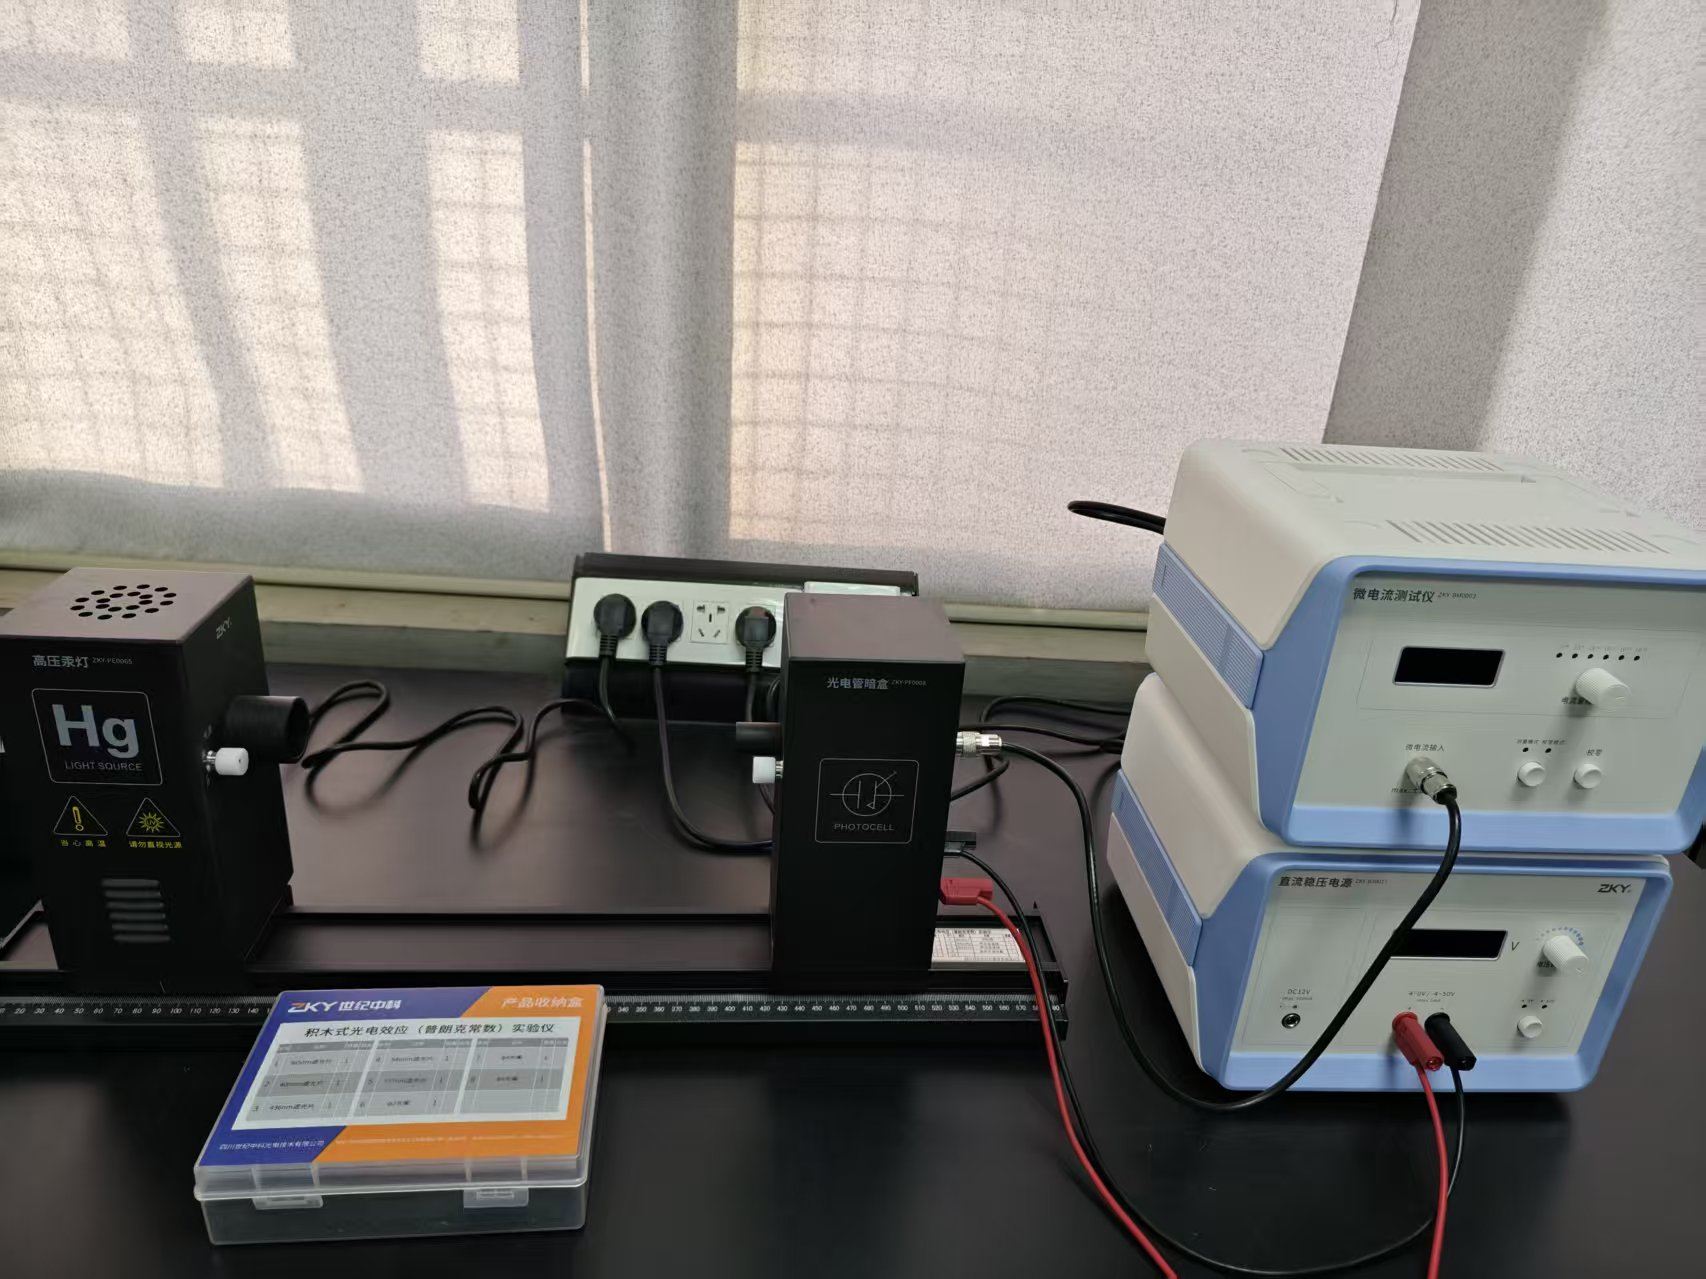
\includegraphics[width=0.8\textwidth]{equipment.jpg}
    \caption{光电效应实验装置示意图}
    \label{fig:fig1}
\end{figure}

\begin{center}
\begin{longtable}{|c|c|c|c|c|}
    \caption{光电效应实验仪器设备清单} \\
    \hline
    序号 & 编码 & 名称 & 数量 & 备注 \\
    \hline
    \endfirsthead
    \hline
    序号 & 编码 & 名称 & 数量 & 备注 \\
    \hline
    \endhead
    1 & BM0003 & 微电流测试仪 & 1 & 含电源线  \\
    \hline
    2 & BJ0011 & 直流稳压电源 & 1 & 含电源线 \\
    \hline
    3 & PF0008 & 光电管暗盒 & 1 &  \\
    \hline
    4 & PE0065 & 高压汞灯 & 1 & 含汞灯电源 \\
    \hline
    5 & BB0011 & 导轨 & 1 & 600mm \\
    \hline
    6 &  & 滤光片光阱收纳盒 & 1 & \makecell[l]{滤光片 365nm、405nm、436nm、546nm、577nm; \\ 光阱 φ2、φ4、φ8} \\
    \hline
    7 & BA0057 & 同轴线 & 1 & \makecell[l]{两端 TNC 内螺纹头，\\线长 500mm} \\
    \hline
    8 & BA0045 & 单芯连接线 & 1 & \makecell[l]{两端 4mm 高压头，\\线长 500mm，红色} \\
    \hline
    9 & BA0046 & 单芯连接线 & 1 & \makecell[l]{两端 4mm 高压头，\\线长 500mm，黑色} \\
    \hline
\end{longtable}
\end{center}

\section{实验原理}
\subsection{光电效应}
入射光照射在光电管的阴极 K 上，产生的光电子在电场的作用下向阳极 A 迁徙构成光电流。改变外加电压 $U_{AK}$ ，测量光电流 $I$ 的大小，即可得出光电管的伏安特性曲线。

按照爱因斯坦的光量子理论，频率为 $\nu$ 的光子具有能量 $E=h\nu$，其中 $h$ 为普朗克常数。当光子照射到金属表面时，被金属中的电子全部吸收，而无需积累能量的时间。电子把这能量的一部分用来克服金属表面对它的吸引力，余下的就变为电力离开金属表面后的动能，按照能量守恒定律，有光电效应方程：
\begin{equation}
    h\nu=\frac{1}{2}mv_0^2+A
\end{equation}
式中，$\frac12 mv_0^2$为光电子获得的初始动能，$m$ 为电子质量，$v_0$ 为最大速度，$A$ 为金属的逸出功，$\nu$ 为光的频率，$h$ 为普朗克常数。由该式可见，入射到金属表面的光频率越高，逸出的电子动能越大，所以即使阳极电位比阴极电位低时也会有电子落入阳极形成光电流，直到阳极电位低于截止电压，光电流才为零，此时有光系：
\begin{equation}
    eU_0=\frac{1}{2}mv_0^2
\end{equation}

阳极电位高于截止电压后，随着阳极电位的升高，阳极对阴极发射收集作用越强，光电流随之上升，当阳极电压高到一定程度，已把阴极发射的光电子几乎全部收集到阳极，再增加 $U_{AK}$ 时 $I$ 不再变化，光电流出现饱和，饱和光电流 $I_M$ 的大小与入射光的强度 $P$ 成正比。

光子的能量 $h\nu_0 <A$，时电子不能脱离金属，因而没有光电流产生，产生光电效应的最低频率（截至频率）是 $\nu_0=A/h$ 。可以得到
\begin{equation}
    eU_0=h\nu-A
\end{equation}
此式表明截止电压 $U_0$ 是频率 $\nu$ 的线性函数，斜率为 $h/e$ ，截距为 $-A/e$ 。通过测量不同频率光照射下的截止电压 $U_0$ ，作出 $U_0-\nu$ 图象，测出斜率和截距，即可求出普朗克常数 $h$ 和金属的逸出功 $A$ 。


\subsection{影响准确测量截至电压的因素}
测量普朗克参数 $h$ 的关键是正确的测出截止电压 $U_0$。但实际上由于光电管制作工艺等原因，给准确认定截止电压带来了困难。暗电流、本底电流和反向电流是对测量产生影响的主要因素。

1）无光照时，也会产生电流，称为暗电流。它由阴极在常温下的热电子发射形成的热电流和封闭在暗盒里的光电管在外加电压下因管子阴极和阳极间绝缘电阻漏电而产生的漏电流两部分组成。

2）本底电流是周围散光进入光电管所致。

3）反向电流是由于制作光电管时阴极上往往混有阳极材料，所以当光照射到阳极上和杂散光漫射到阳极上时，阳极上往往也有光电子发射。此外，阴极发射的光电子也可能被阳极的表面吸引。当阳极A为负电势，阴极K为正电势时，对阴极K上发射的光电子有减速作用，而对阳极A发射或反射的光电子起加速作用，使阳极A发射出的光电子也到达阴极K，形成反向电流。

由于上述原因，实测的伏安特性曲线与理论曲线有区别。
\begin{figure}[H]
    \centering
    
\includegraphics[width=0.6\textwidth]{fig2.png}
    \caption{光电流曲线分析}
    \label{fig:fig2}
\end{figure}

\section{仪器介绍}
\subsection{实验装置}
实验装置由汞灯及电源、滤色片、光阑、光电管、导轨等构成。其中汞灯包含汞灯盒体和电源两部分，光电管安装在光电管暗盒内，暗盒和汞灯分布安装在导轨两侧，可沿滑槽左右移动以改变二者间距离。
\begin{figure}[h]
    \centering
    
\includegraphics[width=0.8\textwidth]{fig3.png}
    \caption{实验装置示意图图}
    \label{fig:fig3}
\end{figure}

汞灯盒与光电管暗盒都设计有通光开关，在仪器不使用，不进行测试时，需要将两个开关都置于“关”状态。

\subsection{微电流测试仪}
\begin{figure}[h]
    \centering
    
\includegraphics[width=0.6\textwidth]{fig4.png}
    \caption{微电流测试仪面板示意图}
    \label{fig:fig4}
\end{figure}
微电流测试仪在该实验中，主要测试的是光电管的微弱电流。该实验测试前及切换电流量程后，都需要进入校零模式进行校零操作。

\subsection{直流稳压电源}
\begin{figure}[h]
    \centering
    
\includegraphics[width=0.6\textwidth]{fig5.png}
    \caption{直流稳压电源面板示意图}
    \label{fig:fig5}
\end{figure}

直流稳压电源在该实验系统中，主要为光电管提供偏置电压。有两个电压输出档位，分别为 $-4.000\sim 0 \mathrm{V}$ 档和 $-4.0\sim 50.0\mathrm {V}$ 档。

\section{实验内容与步骤}

\subsection{实验前准备}
1）首先确保汞灯及光电管暗盒通光开关处于“关”，然后将测试仪及汞灯电源接通，预热＞20分钟。

2）将汞灯光输出口对准光电管暗盒光输入口，调整光电管与汞灯距离为约\textbf{40cm}。

3）用专用单芯连接线将光电管暗盒电压输入端与直流稳压电源输出端连接起来（红—红，黑—黑）。

4）用专用同轴线将光电管暗盒与微电流测试仪输入端连接起来。

5）\textbf{校零}：汞灯及光电管暗盒通光开关都处于“关”，将电流量程选择开关置于所需测试档位，仪器在充分预热后，进行测试仪校零。校零时，通过模式切换按键，使校零模式小数点亮状态；当表头显示稳定后，按下“校零”按键，使电流指示为“00.0”。调节好后，通过模式切换按键切换到“测试模式”，就可以进行实验了。

	\textbf{注意1：}在进行每一组实验前，每一次切换电流量程档位后，都必须进行校零，否则影响实验精度。

	\textbf{注意2：}在仪器使用过程中，汞灯不宜直接照射光电管，也不宜长时间连续照射有功光阑和光电管的光电管，如此将减少光电管的使用寿命。实验完成后，请将光电管通光开关处于“关”状态。


\subsection{测量普朗克常数 $h$}
本仪器采用新型结构的光电管，使得阳极反向电流大大降低，暗电流也很弱。因此，在测量截止电压 $U_0$ 时，可以直接采用“零电流法”。

\subsubsection{测量}
将电压选择按键置于 -4 V～0 V 档，“电流量程”$10^{-12}$ A 档位，将仪器按照前面方法校零；汞灯、光电管间距 40cm；使用直径 4mm 的光阑及 365.0nm 的滤色片，打开汞灯通光口（开关处于“开”）。

	\textbf{注意：}光阑及滤光片调整好后，再打开汞灯通光开关（适用于后文所有相同的实验操作）。

从低到高调节电压，用“零电流法”测量该波长对应的 $U_0$，并将数据记录于 Table 2 中。
依次换上 404.7nm、435.8nm、546.1nm、577.0nm 的滤色片，重复以上测量步骤。

\begin{table}[H]
    \centering
    \caption{截止电压的测试表（$U_0-\nu$ 关系）}
    \vspace{2pt}
    \begin{minipage}{0.9\textwidth}
        \raggedleft
        光阑 $\Phi=40$ mm
    \end{minipage}\\[2pt]
    \begin{tabular}{cccccc}
        波长 $\lambda$(nm) & 365.0 & 404.7 & 435.8 & 546.1 & 577.0 \\
        \hline \hline
        频率 $\nu$ ($\times 10^{14}$ Hz) & 8.214 & 7.405 & 6.879 & 5.490 & 5.196 \\
        \hline
        截止电压 $U_0$ (V)& -1.647& -1.318& -1.135& -0.5747& -0.462 \\
    \end{tabular}
\end{table}

\subsubsection{数据处理}
处理 Table 2 数据，得出 $U_0-\nu$ 直线的斜率 $k$，即可用 $h=ek$ 求出普朗克常数，并与公认值 $h_0$ 比较求出相对误差 $E=\frac{|h-h_0|}{h_0}$，其中 $e=1.602\times 10^{-19}\ \mathrm{C}$，$h_0=6.626\times 10^{-34}\ \mathrm{J\cdot s}$。计算逸出功 $A$ 与截止频率 $\nu_0$。
\begin{figure}[h]
    \centering
    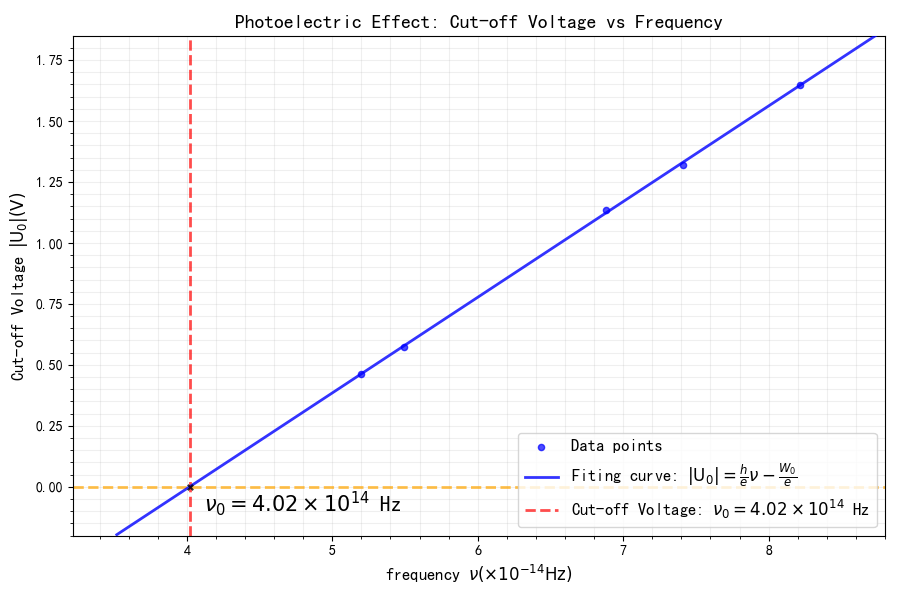
\includegraphics[width=1\textwidth]{Figure_1.png}
    \caption{$U_0-\nu$ 关系图}
    \label{fig:fig6}
\end{figure}

拟合曲线得到$|U_0| = (3.922e-15 ± 3.997e-17)\nu + (-1.576 ± 0.027)$ 。可以得到:
$$
普朗克常数\ h = 6.283 \times 10^{-34} J·s 
$$
$$
相对误差\ E=5.17\%
$$
$$
逸出功\ A = 2.525\times 10^{-19}\ J
$$
$$
截止频率\ \nu_0 = 4.02\times 10^{14}\ Hz
$$



\subsection{测量光电管的伏安特性曲线}
a.将电压置于-4V～50V档，“电流量程”$10^{-11}$A档位，且将仪器按照前面方法校零；汞灯、光电管间距40cm；选择“$\Phi 4$”光阑及“356”滤色片，打开汞灯暗盒开始实验。从低到高调节节电压，记录相应的电流，电压值作为第一组数据，以后电压每变化一定值记录一组数据到 Table 3 中；选择“$\Phi 4$”光阑及其他四种滤色片重复a中测量步骤；用 Table 3 数据作出对应于不同波长的伏安特性曲线。

\begin{table}[H]
    \centering
    \caption{I-$U_{AK}$ 关系}
    \vspace{2pt}
    \begin{minipage}{0.9\textwidth}
        \centering
        $L$= 400 mm \hspace{1cm} $\Phi$= 40 mm
    \end{minipage}\\[2pt]
    \small
    \begin{tabular}{c|cccccccccc}
    波长$\lambda\ (\mathrm{nm})$     & $U_{AK}\ (\mathrm{V})$                       & -1   & 0    & 1    & 5    & 10    & 15    & 20    & 25   & 30   \\ \hline \hline
    365.0 & $I (\times 10^{-11}\ \mathrm A)$  & 8.5  & 36.4 & 67.2 & 215  & 350   & 471   & 570   & 652  & 711  \\ \hline
    404.7 & $I (\times 10^{-11}\ \mathrm A)$ & 1.4  & 11   & 23.5 & 70.7 & 113.2 & 151.6 & 181.2 & 205  & 220  \\ \hline
    435.8 & $I (\times 10^{-11}\ \mathrm A)$ & 2.1  & 30.4 & 68.2 & 195  & 309   & 408   & 482   & 538  & 569  \\ \hline
    546.1 & $I (\times 10^{-11}\ \mathrm A)$ & 0.1  & 2.3  & 7.7  & 21.9 & 31.4  & 37.5  & 40.8  & 43.1 & 44.2 \\ \hline
    577.0 & $I (\times 10^{-11}\ \mathrm A)$ & -0.1 & 0.9  & 4.2  & 11.8 & 16.7  & 19.5  & 21    & 22.1 & 22.8 \\ 
    \end{tabular}
\end{table}

\textbf{注意：}为避免光电管长时间处于较高电压下加速光电管老化，伏安特性这里的实验应快速完成。

\begin{figure}[H]
    \centering
    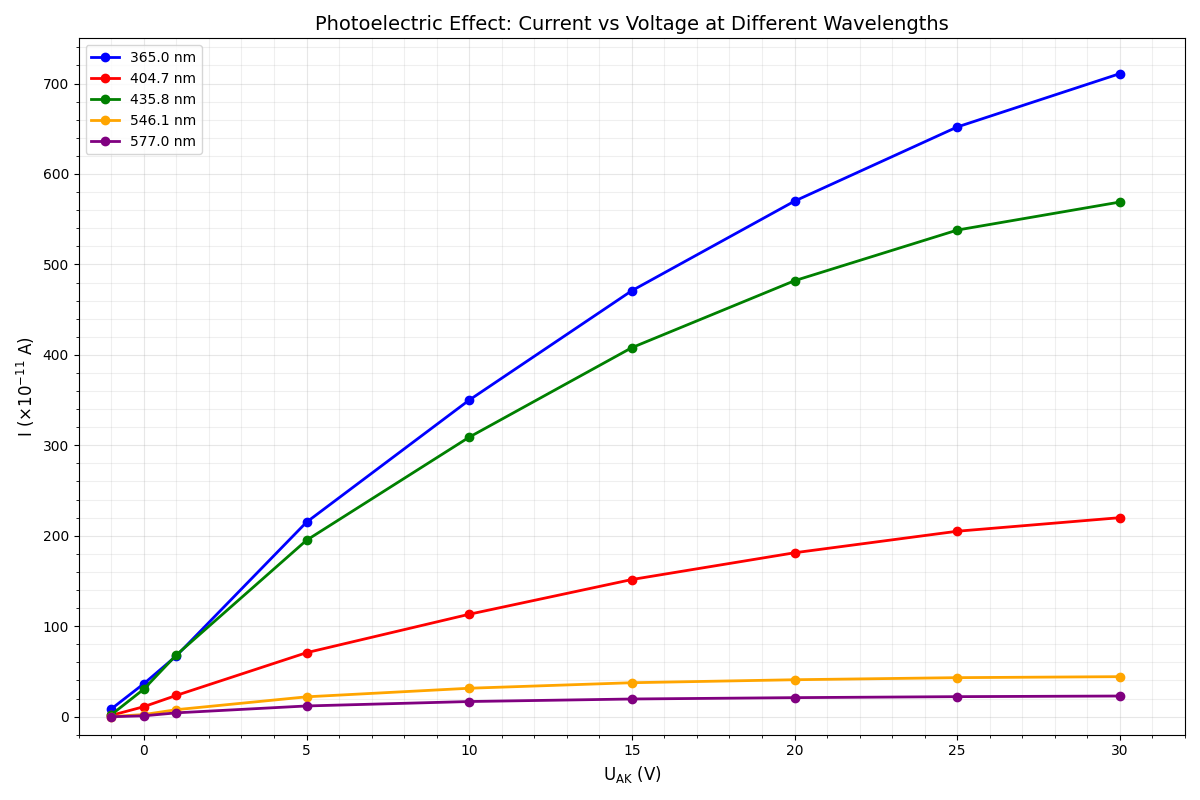
\includegraphics[width=1\textwidth]{Figure_2.png}
    \caption{光电管伏安特性曲线}
    \label{fig:fig7}
\end{figure}

b.将 $U_{AK}$ 设置为 30V 时，将“电流量程”选择开关置于$10^{-10}$A 档，将仪器按照前面方法校零，在同一谱线，同一入射距离下下，记录光阑分别为“$\Phi 2$”，“$\Phi 4$”，“$\Phi 8$”时对应的电流值于 Table 4 中，由于照到光电管上的光强于光阑面积成正比，用 Table 4 数据验证光电管的饱和光电流与入射光强成正比。

\begin{table}[H]
    \centering
    \caption{$I_M - P$关系表}
    \vspace{2pt}
    \begin{minipage}{0.9\textwidth}
        \centering
        $L$= 400 mm \hspace{1cm} $U_{AK}$= 30 V
    \end{minipage}\\[2pt]
    \begin{tabular}{c|cccc}
    波长$\lambda$(nm)    & $\Phi$             & 2mm  & 4mm  & 8mm  \\ \hline \hline
    435.8 & $I (\times 10^{-10}\ \mathrm A)$  & 15.9 & 56.9 & 208  \\ \hline
    546.1 & $I (\times 10^{-10}\ \mathrm A)$  &1.3 & 4.5  & 16.5  
    \end{tabular}
\end{table}

可以看到，在误差允许的范围内，光电流与光阑面积成正比。

\section{思考题}
1.光电效应有哪些实际应用？请选择其中一个简要解释其工作原理是如何建立在光电效应的基础上的。

实际应用：光电管和光电传感器、太阳能电池，光电成像器件。光电传感器接收到光线时，内部材料发生光电效应，从而产生电信号，实现对光的感知。

2.$U_0-\nu$ 图中直线的斜率和截距的物理意义是什么？如果更换另一种阴极材料，图像可能会发生什么变化？

斜率的物理意义时 $h/e$ ，其中 $h$ 是普朗克常数，$e$ 是电子电量，截距是 $-A/e$ ， $A$ 是金属的逸出功。更换另一种阴极材料，图象的斜率不发生改变，截距发生改变。 

3.在实验过程中，固定入射光的频率，观察光电流随外加电压的变化（即 $I-U$ 图）。当电压为负值（反向电压）时，为什么光电流不会突然降为零，而是随着反向电压增大逐渐减小？电压为正值且不断增大时，光电流为什么会达到一个“饱和值”？

因为不同的光电子有不同的初动能，速度的方向也不一样，所以光电流会随着方向电压的增大逐渐减小。但电压为正值且不断增大时，几乎所有的光电子都可以到达阳极形成光电流，所以光电流会达到一个饱和值。

\end{document}

